\chapter{Conclusiones}

\section{Conclusiones Generales}
    
    La práctica fue concluida con satisfacción, ya que nos resultó bastante didactico el modo de emplear un algoritmo tan común como el de Fibonacci para hacer un análisis certero de su rendmiento temporal. 
    
    Tuvimos complicaciones en la ejecución de los algoritmos porque queriamos medir su complejidad con cantidades muy grandes de números, presentando así problemas para poder continuar con la ejecución de los algoritmos.
    
    Comprendimos de mejor manera un análisis a priori a un algoritmo iterativo. 

\newpage
\section{Isaac Sánchez - Conclusiones}
    Esta práctica me permtió desarrollar mis habilidades a la hora de realizar algoritmos recursivos, ya que es un concepto que no dominaba. De igual manera, el análisis en la parte de priori fue más sencilla de plasmar para dar una idea. Mis conceptos que aprendí de mejor manera fue: recursividad y como encontrar un número perfecto.
    \begin{figure}[htp!]
            \centering
            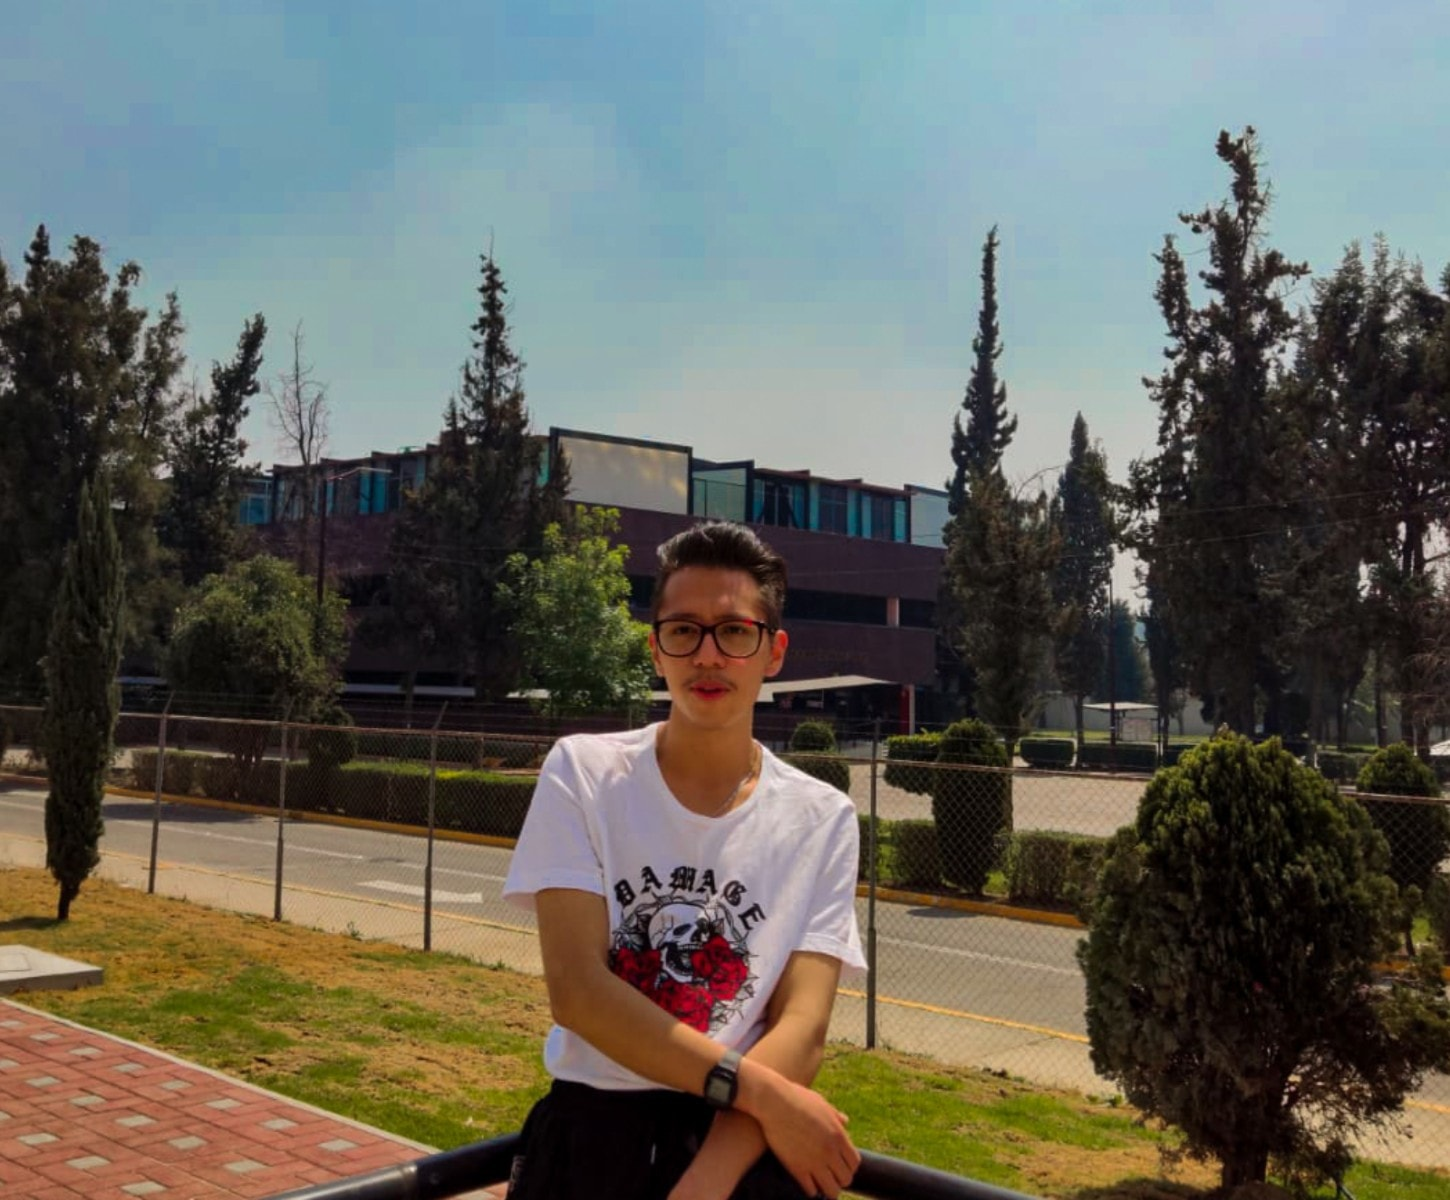
\includegraphics[width=1 \textwidth]{Images/Fotos_Alumnos/274612600_2528992867236334_6677874837890685705_n.jpg}  
            \caption{Isaac Sánchez}
            \label{fig:my_label1}
        \end{figure}
    


\newpage
\section{Axel Trevino - Conclusiones}
    Durante esta práctica vimos que la recursividad no siempre es buena, ya que en el de Fibonacci aparte de necesitar más optimización no pudimos correrlo con números grandes porque causábamos un stack overflow
    \begin{figure}[htp!]
            \centering
            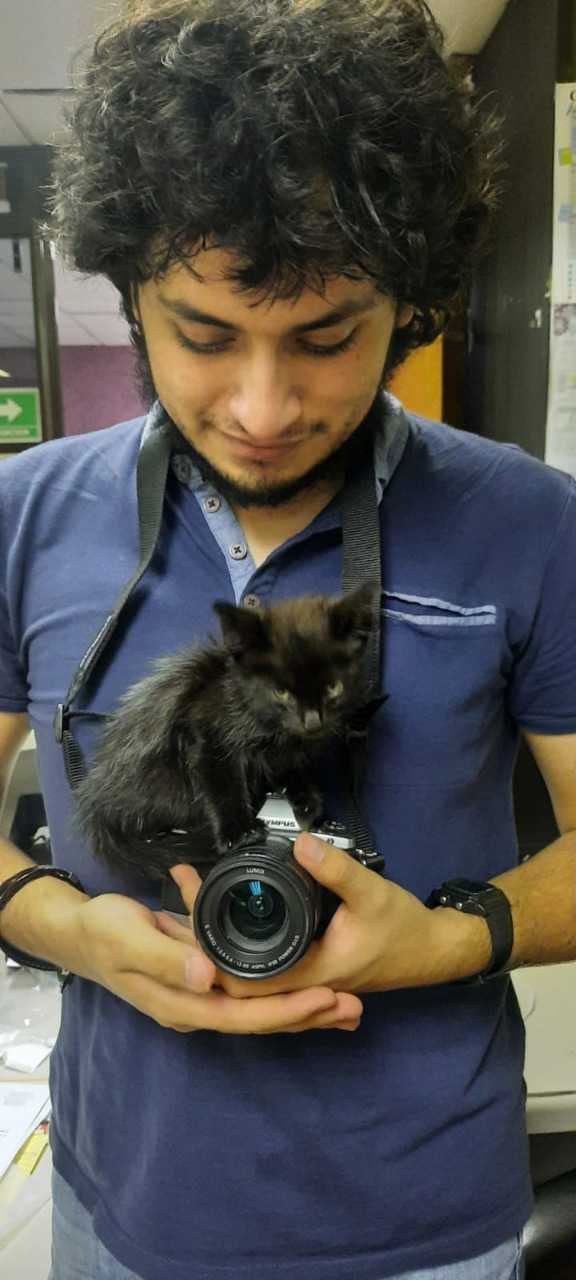
\includegraphics[width=0.4 \textwidth]{Images/Fotos_Alumnos/axel.jpg}  
            \caption{Axel Treviño}
            \label{fig:my_label2}
        \end{figure}
